
\documentclass[review]{elsarticle}
\usepackage{hyperref}
\usepackage[margin=1in]{geometry}
\usepackage{graphicx}
\usepackage{amsmath}
\usepackage{placeins}
\usepackage{comment}
\usepackage{textcomp}
\usepackage{gensymb}
\usepackage{lineno}
\usepackage{color}
\usepackage{cleveref}
\usepackage{multicol}

\usepackage[utf8]{inputenc}
\usepackage[english]{babel}

\usepackage[dvipsnames]{xcolor}

%\journal{Journal of Nuclear Materials}
\bibliographystyle{elsarticle-num}

\begin{document}

\begin{frontmatter}

\title{LiCl-KCl-NaCl working title... }

\author[ncsu,inl]{Benjamin Beeler\corref{qwe}}
\cortext[qwe]{Corresponding author}
\author[inl]{Ruchi Gakhar}

\address[ncsu]{North Carolina State University, Raleigh, NC 27695}
\address[inl]{Idaho National Laboratory, Idaho Falls, ID 83415}
\date{\today}

\begin{abstract}
text for abstract

\end{abstract}

\end{frontmatter}

\section{Introduction}

Due to the favorable properties, such as the wide range of thermal stability and chemical and radiochemical stability, molten halides are widely used in electro refining, nuclear waste recycling, and aluminum production applications \cite{rollet2011}. Alkali halides are not only widely used in the electrolysis process, but also in solar storage \cite{Ding2017} and as nuclear coolants \cite{Li2017}. 


Some intro about molten salts/reactors

Info about experimental data for salts

Some intro about computational methods into salts

What work has been done in these systems?

What we will do?

\section{Computational Methods}\label{sec:method}
The AIMD simulations were performed with the VASP code~\cite{Kresse1996}. All simulations used the $\Gamma$ point for integration in reciprocal space. The plane wave cut-off energy was increased above the standard setting to 500 eV, which is 200 eV above the recommended value. Gaussian smearing with a smearing parameter of 0.02 eV was used for the partial occupancies of the wave functions. The convergence criteria for the electronic minimization was at most 10$^{-4}$ eV. The Projector Augmented Wave (PAW) method was used to describe the core electrons~\cite{PAW1,PAW2}. It is well-established in the literature that Van der Waals (vdW), or dispersion, interactions are critical for reproducing the density of molten salts by DFT methods~\cite{Li,Nam2014,Nam2015}. In general, density functional theory methods are unable to describe Van der Waals dispersion forces. A pragmatic method to work around this problem is to add a correction to the conventional Kohn-Sham DFT energy. This is performed through the addition of a vdW correction, or a replacement of the exchange-correlation functional to account for dispersion interactions. Previous simulations have used both the DFT-D3~\cite{Li,Grimme} and the Langreth \& Lundqvist (vdW-DF2)~\cite{Nam2015,Dion,Klimes} methodologies for various molten chloride salts. In this work, the vdW-DF2 functional was utilized to describe vdW dispersion interactions, as it has been shown to accurately reproduce a number of thermophysical properties of the LiCl-KCl system for a wide range of compositions \cite{Duemmler2021}. 

Compositions including the three molecular species, pseudo-binary eutectics, and various ternary compositions are investigated in this work, shown in \cref{fig:ternary}.

\begin{figure}[htbp]
\begin{center}
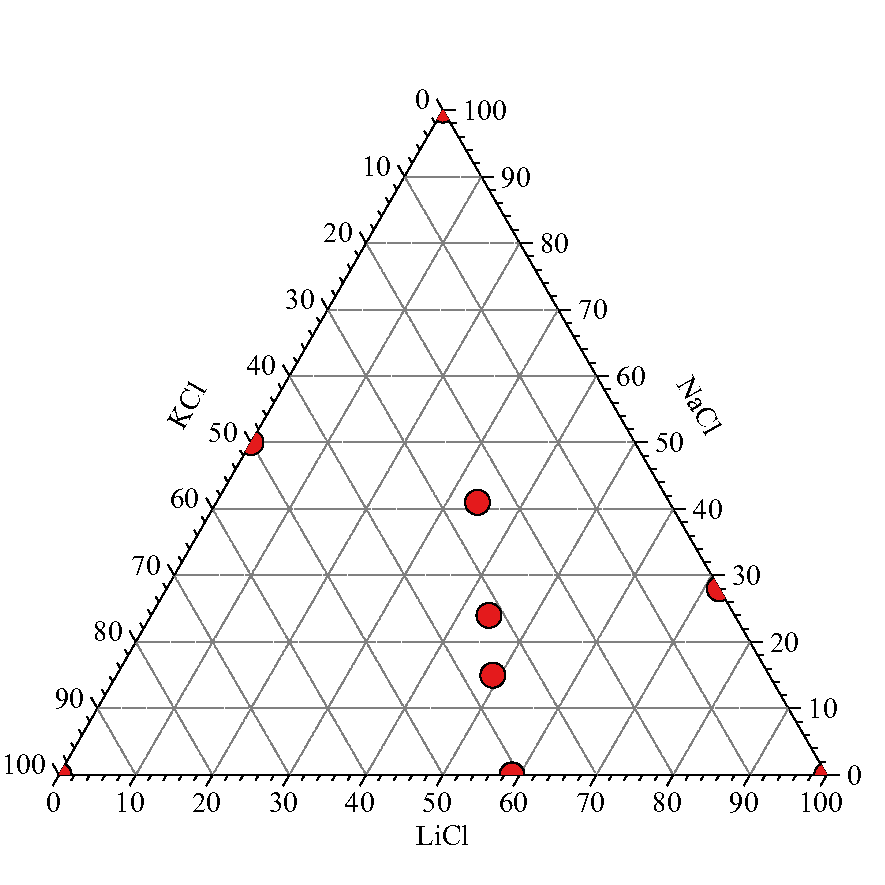
\includegraphics[width=0.75\textwidth]{ternary.pdf}
\caption{Ternary compositions of the LiCl-KCl-NaCl system.}
\label{fig:ternary}
\end{center}
\end{figure}


\FloatBarrier

\section{Results and Discussion}


\begin{figure}[htbp]
\begin{center}
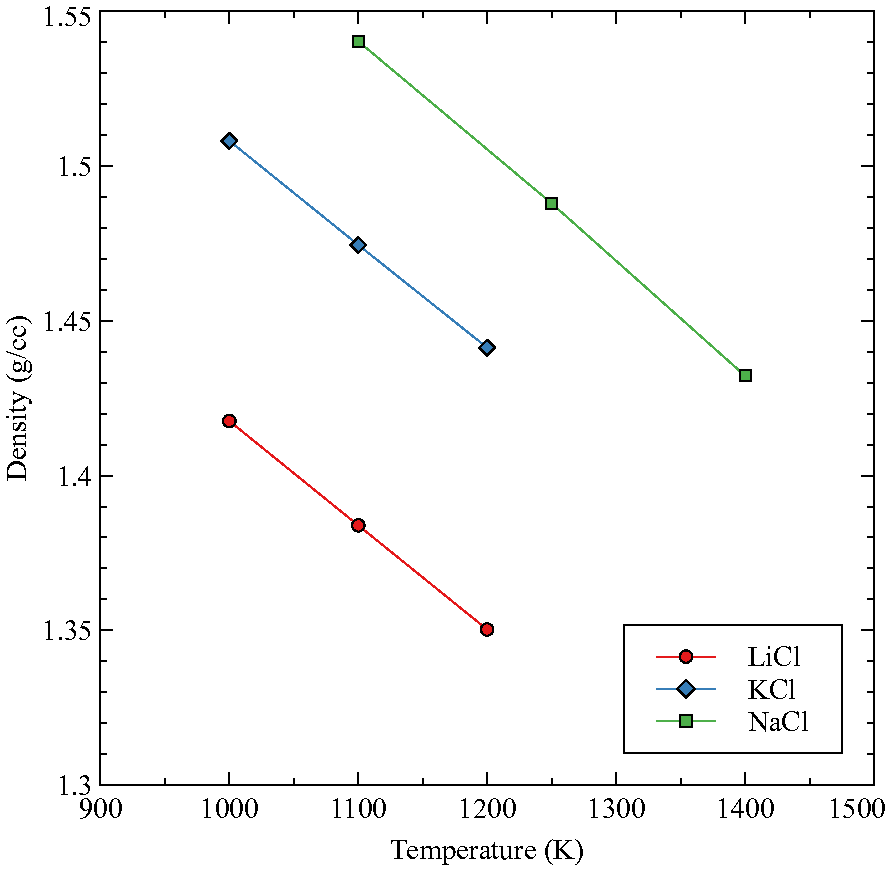
\includegraphics[width=0.75\textwidth]{./images/endpoints.pdf}
\caption{Densities of LiCl, KCl, and NaCl as a function of temperature.}
\label{default}
\end{center}
\end{figure}

\begin{figure}[htbp]
\begin{center}
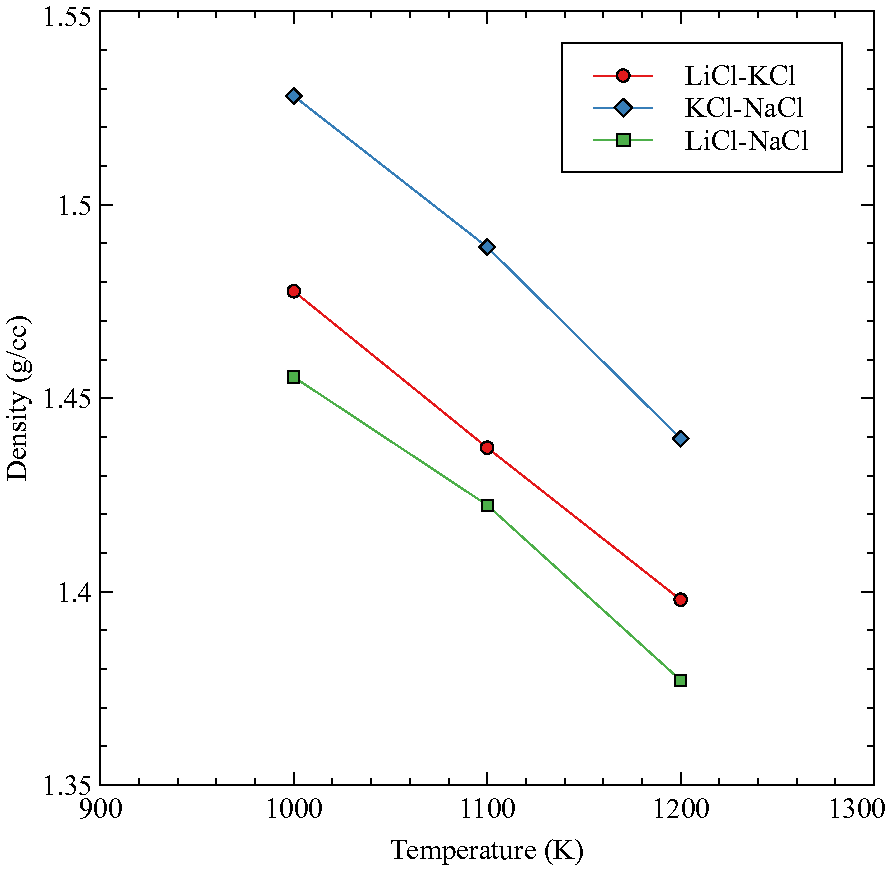
\includegraphics[width=0.75\textwidth]{./images/binaries.pdf}
\caption{Densities of the eutectic compositions of LiCl-KCl, KCl-NaCl, and LiCl-NaCl as a function of temperature.}
\label{default}
\end{center}
\end{figure}



\begin{figure}[htbp]
\begin{center}
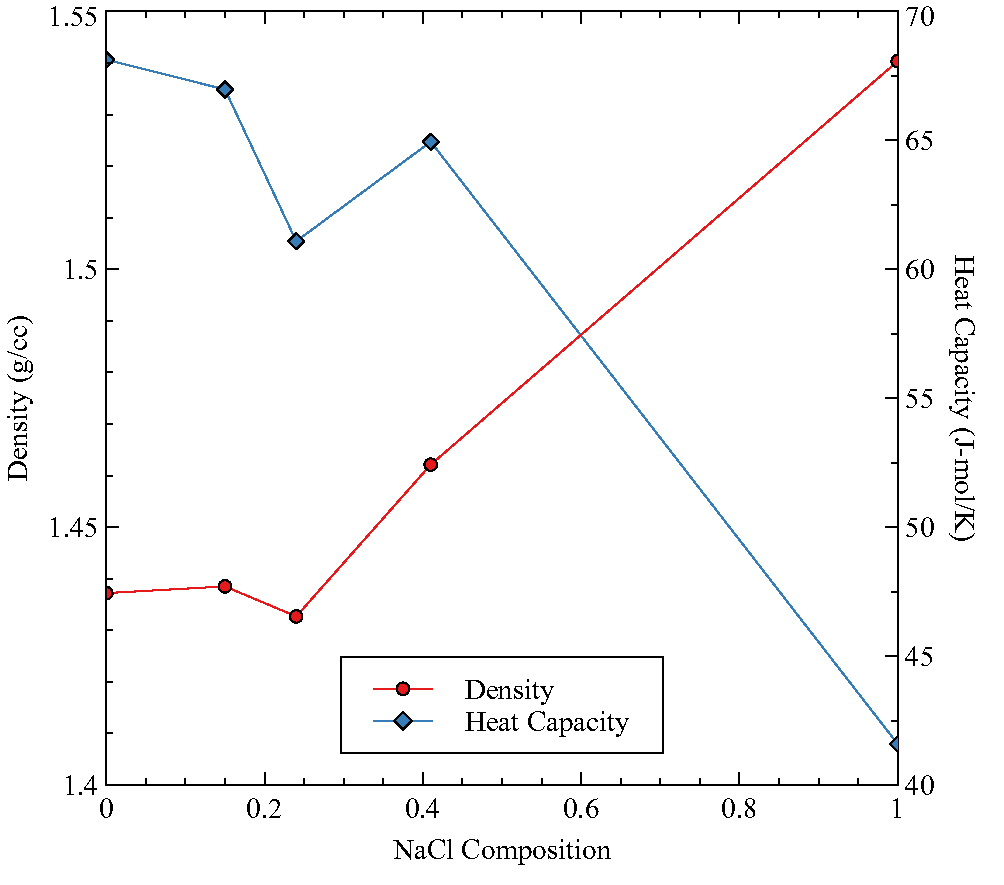
\includegraphics[width=0.75\textwidth]{./images/dens_cp_nacl.pdf}
\caption{Density and heat capacity of the LiCl-KCl-NaCl system at 1100 K as a function of NaCl composition.}
\label{default}
\end{center}
\end{figure}

\FloatBarrier

\section{Conclusions}


\section{Acknowledgements}

This work is supported through the INL Laboratory Directed Research and Development (LDRD) Program under DOE Idaho Operations Office Contract DE-AC07-05ID14517. This research made use of the resources of the High-Performance Computing Center at Idaho National Laboratory, which is supported by the Office of Nuclear Energy of the U.S. Department of Energy and the Nuclear Science User Facilities.  

\bibliography{beeler.bib}

\end{document}
